%************************************************
\chapter{How it works}\label{ch:how_it_works} % $\mathbb{ZNR}$
%************************************************

All code of the examples can be found in the appendix and will not be printed here.

\section{Booking a location}
\label{sec:booking}

To book a location the user has to select a location from the \texttt{DropDown}-box and click the book button:

\begin{figure}[H]
\begin{center}
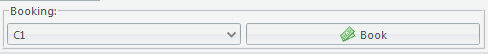
\includegraphics[width=\textwidth]{gfx/booking.png} 
\end{center}
\caption{Booking a location.}
\label{fig:booking}
\end{figure}

This will trigger the \texttt{actionListener} of the \texttt{bookButton} (implemented as an anonymous inner class) that will receive the event from the \texttt{EventDispatcher}-thread.

In the \texttt{actionPerformed}-method the text (equals to the id of the location) of the \texttt{comboBox} will be retrieved and the \texttt{bookLocation}-method of the \texttt{LocationManager} will be invoked with it.

The method will set the \texttt{booked}-flag to true and increase the bookings if the location is not already booked. If the location is already booked an exception will be thrown and an error message displayed by the \ac{GUI}.

If the location is successfully booked, the manager will notify the \ac{GUI} via an \texttt{observer}-pattern, the \ac{GUI} will reload the locations that are displayed and redisplay them - now the flag of the booked location will be coloured red, as it is booked.

\begin{figure}[H]
\begin{center}
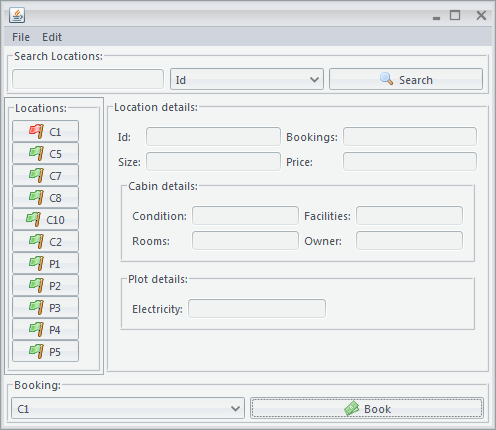
\includegraphics[scale=0.75]{gfx/location_booked.png} 
\end{center}
\caption{Successfully Booked location marked with red flag.}
\label{fig:booked_location}
\end{figure}

A short sequence-diagram of the successful booking looks as follows:

\begin{figure}[H]
\begin{center}
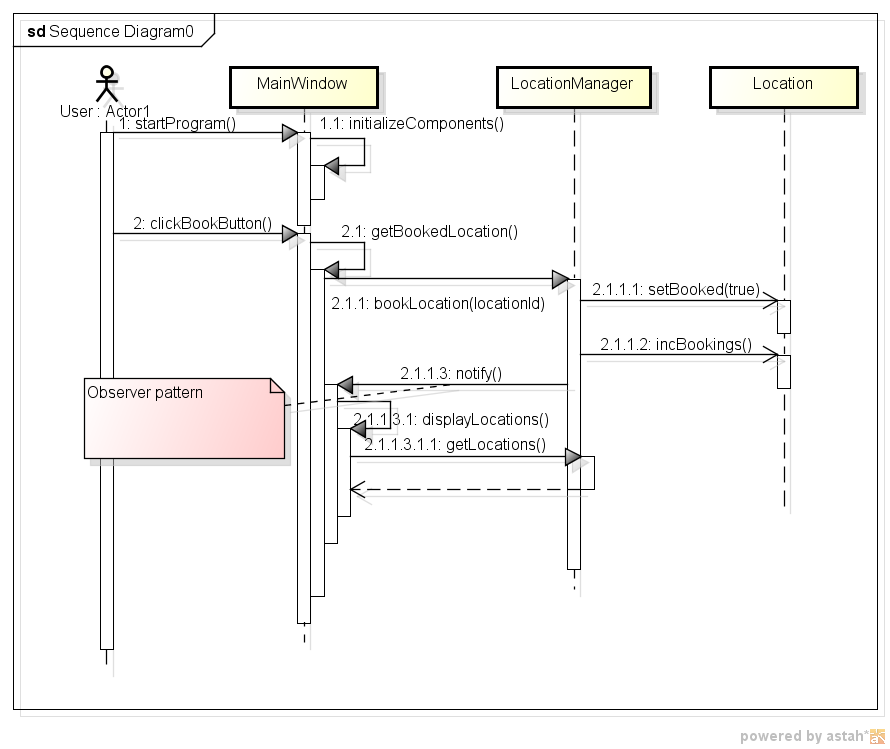
\includegraphics[width=\textwidth]{gfx/booking_sequence.png} 
\end{center}
\caption{Sequence diagram of a successful booking process.}
\label{fig:booking_sequence}
\end{figure}

\section{Display location information}
\label{sec:location_information}

To display a location's information, the user simply clicks on one of the buttons listed in the main \ac{GUI}.

This will trigger the \texttt{actionPerformed}-event of the button that is linked to the \texttt{actionListener} implemented in the \texttt{MainWindow}.

In the actionListener the source of the event is cast to a \texttt{JButton}, the text of the button (equal to a location's id) is read and the \texttt{displayLocation}-method is called with the string \texttt{id}.

The \texttt{displayLocation}-method first retrieves the location associated with the \texttt{id}, then fills out the fields common to cabins and plots (id, bookings, price, size). Then it is determined whether the displayed location is a cabin or plot. According to the result the location is cast to the appropriate type and the remaining fields are filled in.

\begin{figure}[H]
\begin{center}
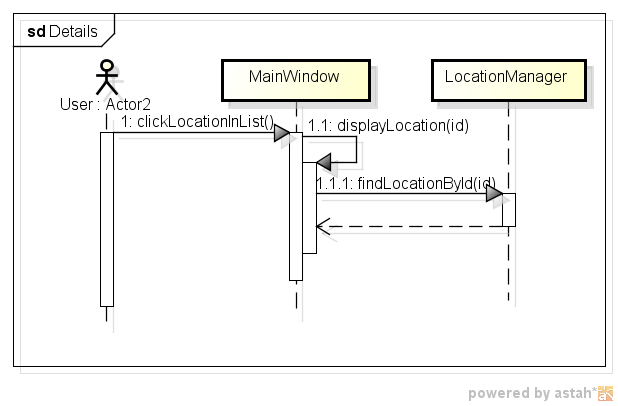
\includegraphics[width=\textwidth]{gfx/details_sequence.png} 
\end{center}
\caption{Sequence diagrams of displaying location details.}
\label{fig:details_sequence}
\end{figure}

\begin{figure}[H]
\begin{center}
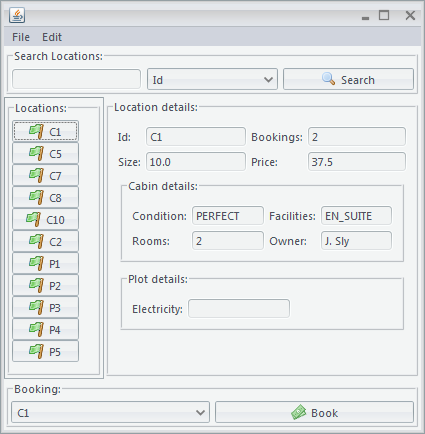
\includegraphics[scale=0.75]{gfx/display_screen.png} 
\end{center}
\caption{Location details are displayed in the gui.}
\label{fig:details_screen}
\end{figure}